\section{Introduction}
Multirobot, autonomous, BLAH BLAH BLAH


\section{MBZIRC Contest}
The contest took place in March in Abu Dhabi. Whole competition consisted of three challenges and the grand challenge which connected all challenges together. The first challenge was the only one which was focused solely on UAVs. The goal of the first challenge was to pop multiple big color balloons and to catch small ball carried by the organizer's drone. The other two challenges was designed for both UGVs and UAVs. The second challenge was about building a wall using the robots. Multiple polystyrene bricks were placed in the arena and the robots should have move these bricks to the destination area and stack them on top of each other to build the wall. Lastly the third challenge was to extinguish fire on the surface of the building model. This task was inspired by fires in the high-rise buildings in UAE. UAVs and UGVs carried tanks full of water and squirt it into the fire dummy.

\subsection{Second challenge}
This thesis is focused on the second challenge and more specifically on the ground robot section of the second challenge, so that we provide more detailed description of this challenge. Each team is given thirty minutes to explore the arena, localize all interest areas and build the wall. There are four types of the bricks with different colors. All bricks must be very light to enable the UAVs to pick them up. The dimension and colors of the bricks can be seen in the figure \ref{fig:brickdef}. 

\begin{figure}[H]

\centering
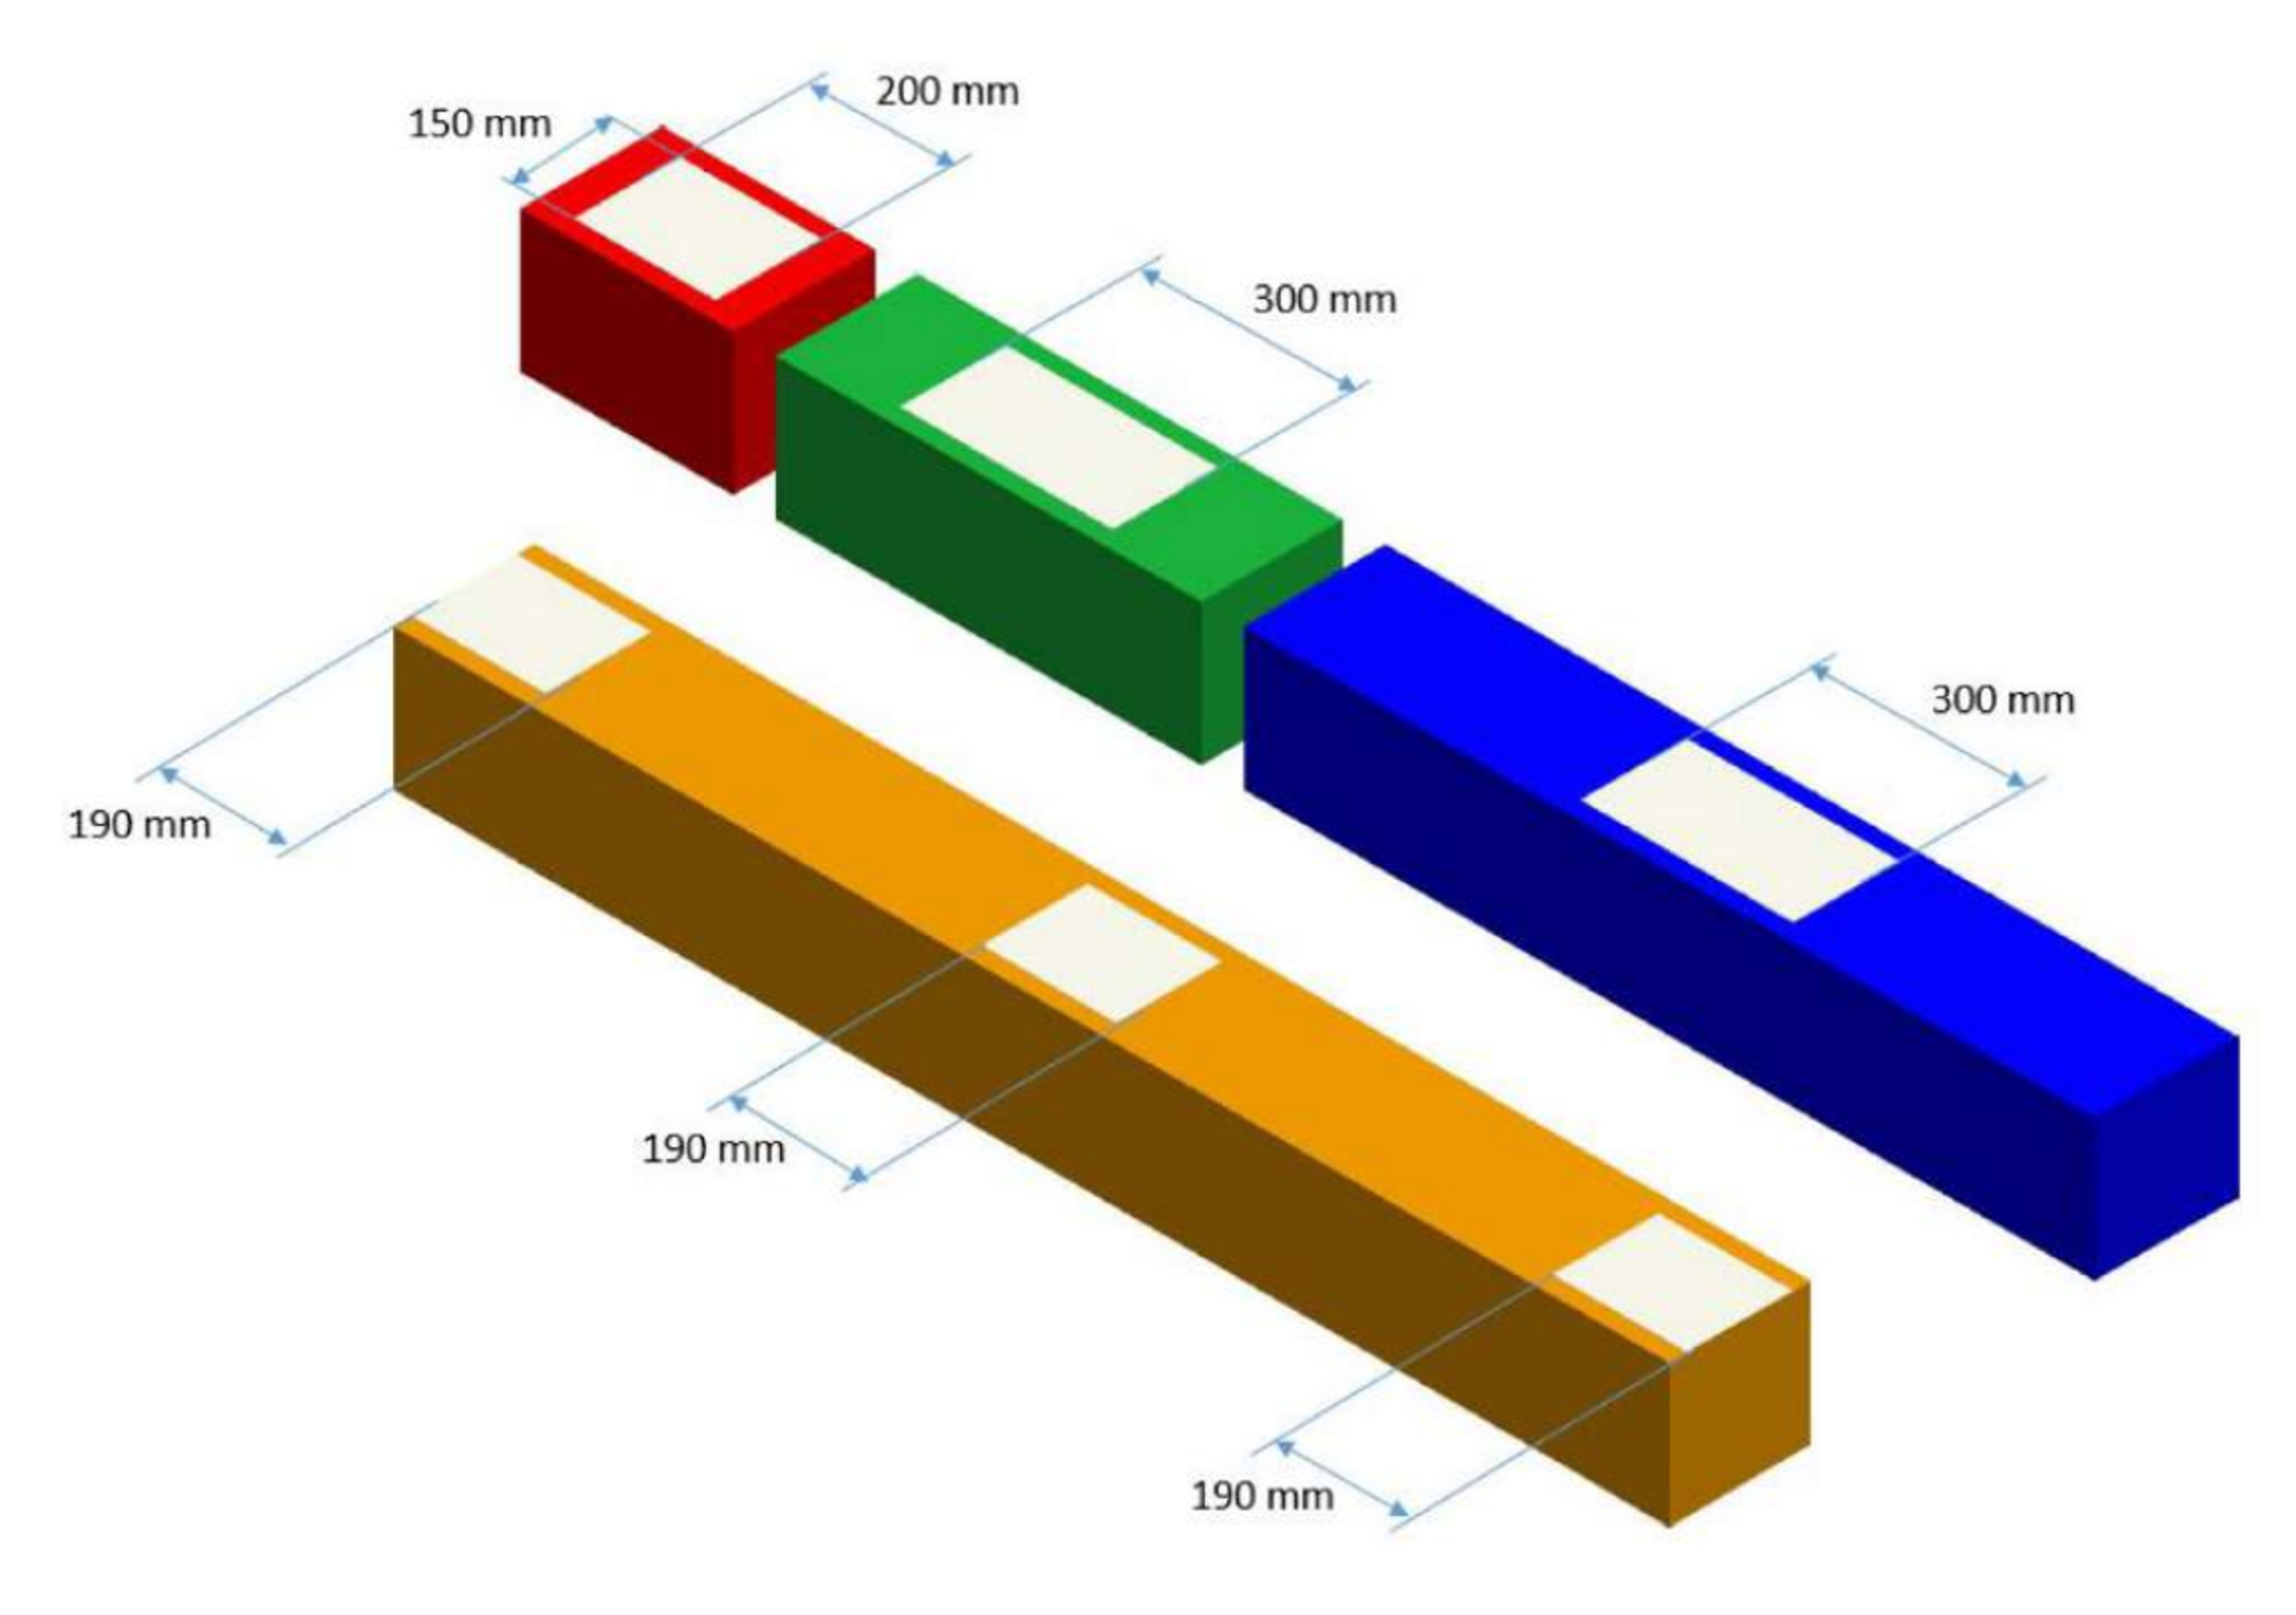
\includegraphics[scale=0.35]{fig/brick_sample.png}
\caption[Bricks definition]{Colors and dimensions of the bricks provided by the organizer.}
\label{fig:brickdef}

\end{figure}

Each brick has thin metal plate on top of it, so that the robots are able to pick them up using electromagnets. In the beginning of challenge are all bricks placed at beforehand unknown position. Initial position of bricks is unknown but there is predefined pattern in which are the bricks put together. There are different patterns for the UGV piles of bricks and the UAV piles. The UGV bricks are stacked into the multiple height levels whereas the UAV bricks are stacked into the width and all are put on the ground. Due to the low weight of the bricks it is necessary to put UAV bricks into the rails, otherwise the bricks can be easily blown away by the propellers of the drones.
